\documentclass{article}
\usepackage[utf8]{inputenc}
\usepackage{graphicx}
\graphicspath{ {images/} }

\title{MIMBCD-UI: Testing Guide}

\author{
  Calisto, Francisco Maria\\
  \texttt{francisco.calisto@tecnico.ulisboa.pt}
}

\date{July 2017}

\begin{document}

\maketitle

\section{Introduction}

This document aims to describe the protocol of the set of tests that will be performed in the scope of the master's thesis of the Medical Imaging Multimodality of Breast Cancer Diagnosis User Interface (MIMBCD-UI) project using a traditional environment (mouse and keyboard). The objective of the tests is to understand the IoU, time performance and error metrics. With the session, the sessions will be recorded via video on the computer and using a record, heat-map and triggered event tools. It is guaranteed the confidentiality of the recordings, which will be used only for academic purposes.

Each test session is divided into three parts. In one test the traditional environment supported by the interaction with mouse and keyboard. The second part, we will do a small questionnaire about experience and feel. Finally, the third part we will have a final questionnaire about preferences of use.

\section{Material}

The material used in the test sessions for the user interface consists of:

\begin{itemize}
  \item MacBook Pro: it will allow the user to interact with the keyboard and a wireless mouse;
  \item Wireless Mouse: it will allow the user to interact with a mouse and will complement the keyboard;
\end{itemize}

\section{Technical Description}

To produce this traditional environment, and since we can simulate with a laptop, the mouse and keyboard interaction, we are using a Microsoft Mobile Mouse 4000 together the MacBook Pro (Retina, 13-inch, Early 2015) with a standard integrated key board on the laptop.

\section{Traditional Environment}

Traditional interaction remains the most common way to interact with user interfaces on a clinical environment. Unfortunately most of this interaction is made by low profile equipment that make users produce more errors and take more time interacting with those user interfaces.

\begin{figure}[h]
\caption{Example of a Freehand ROI Annotation}
\centering
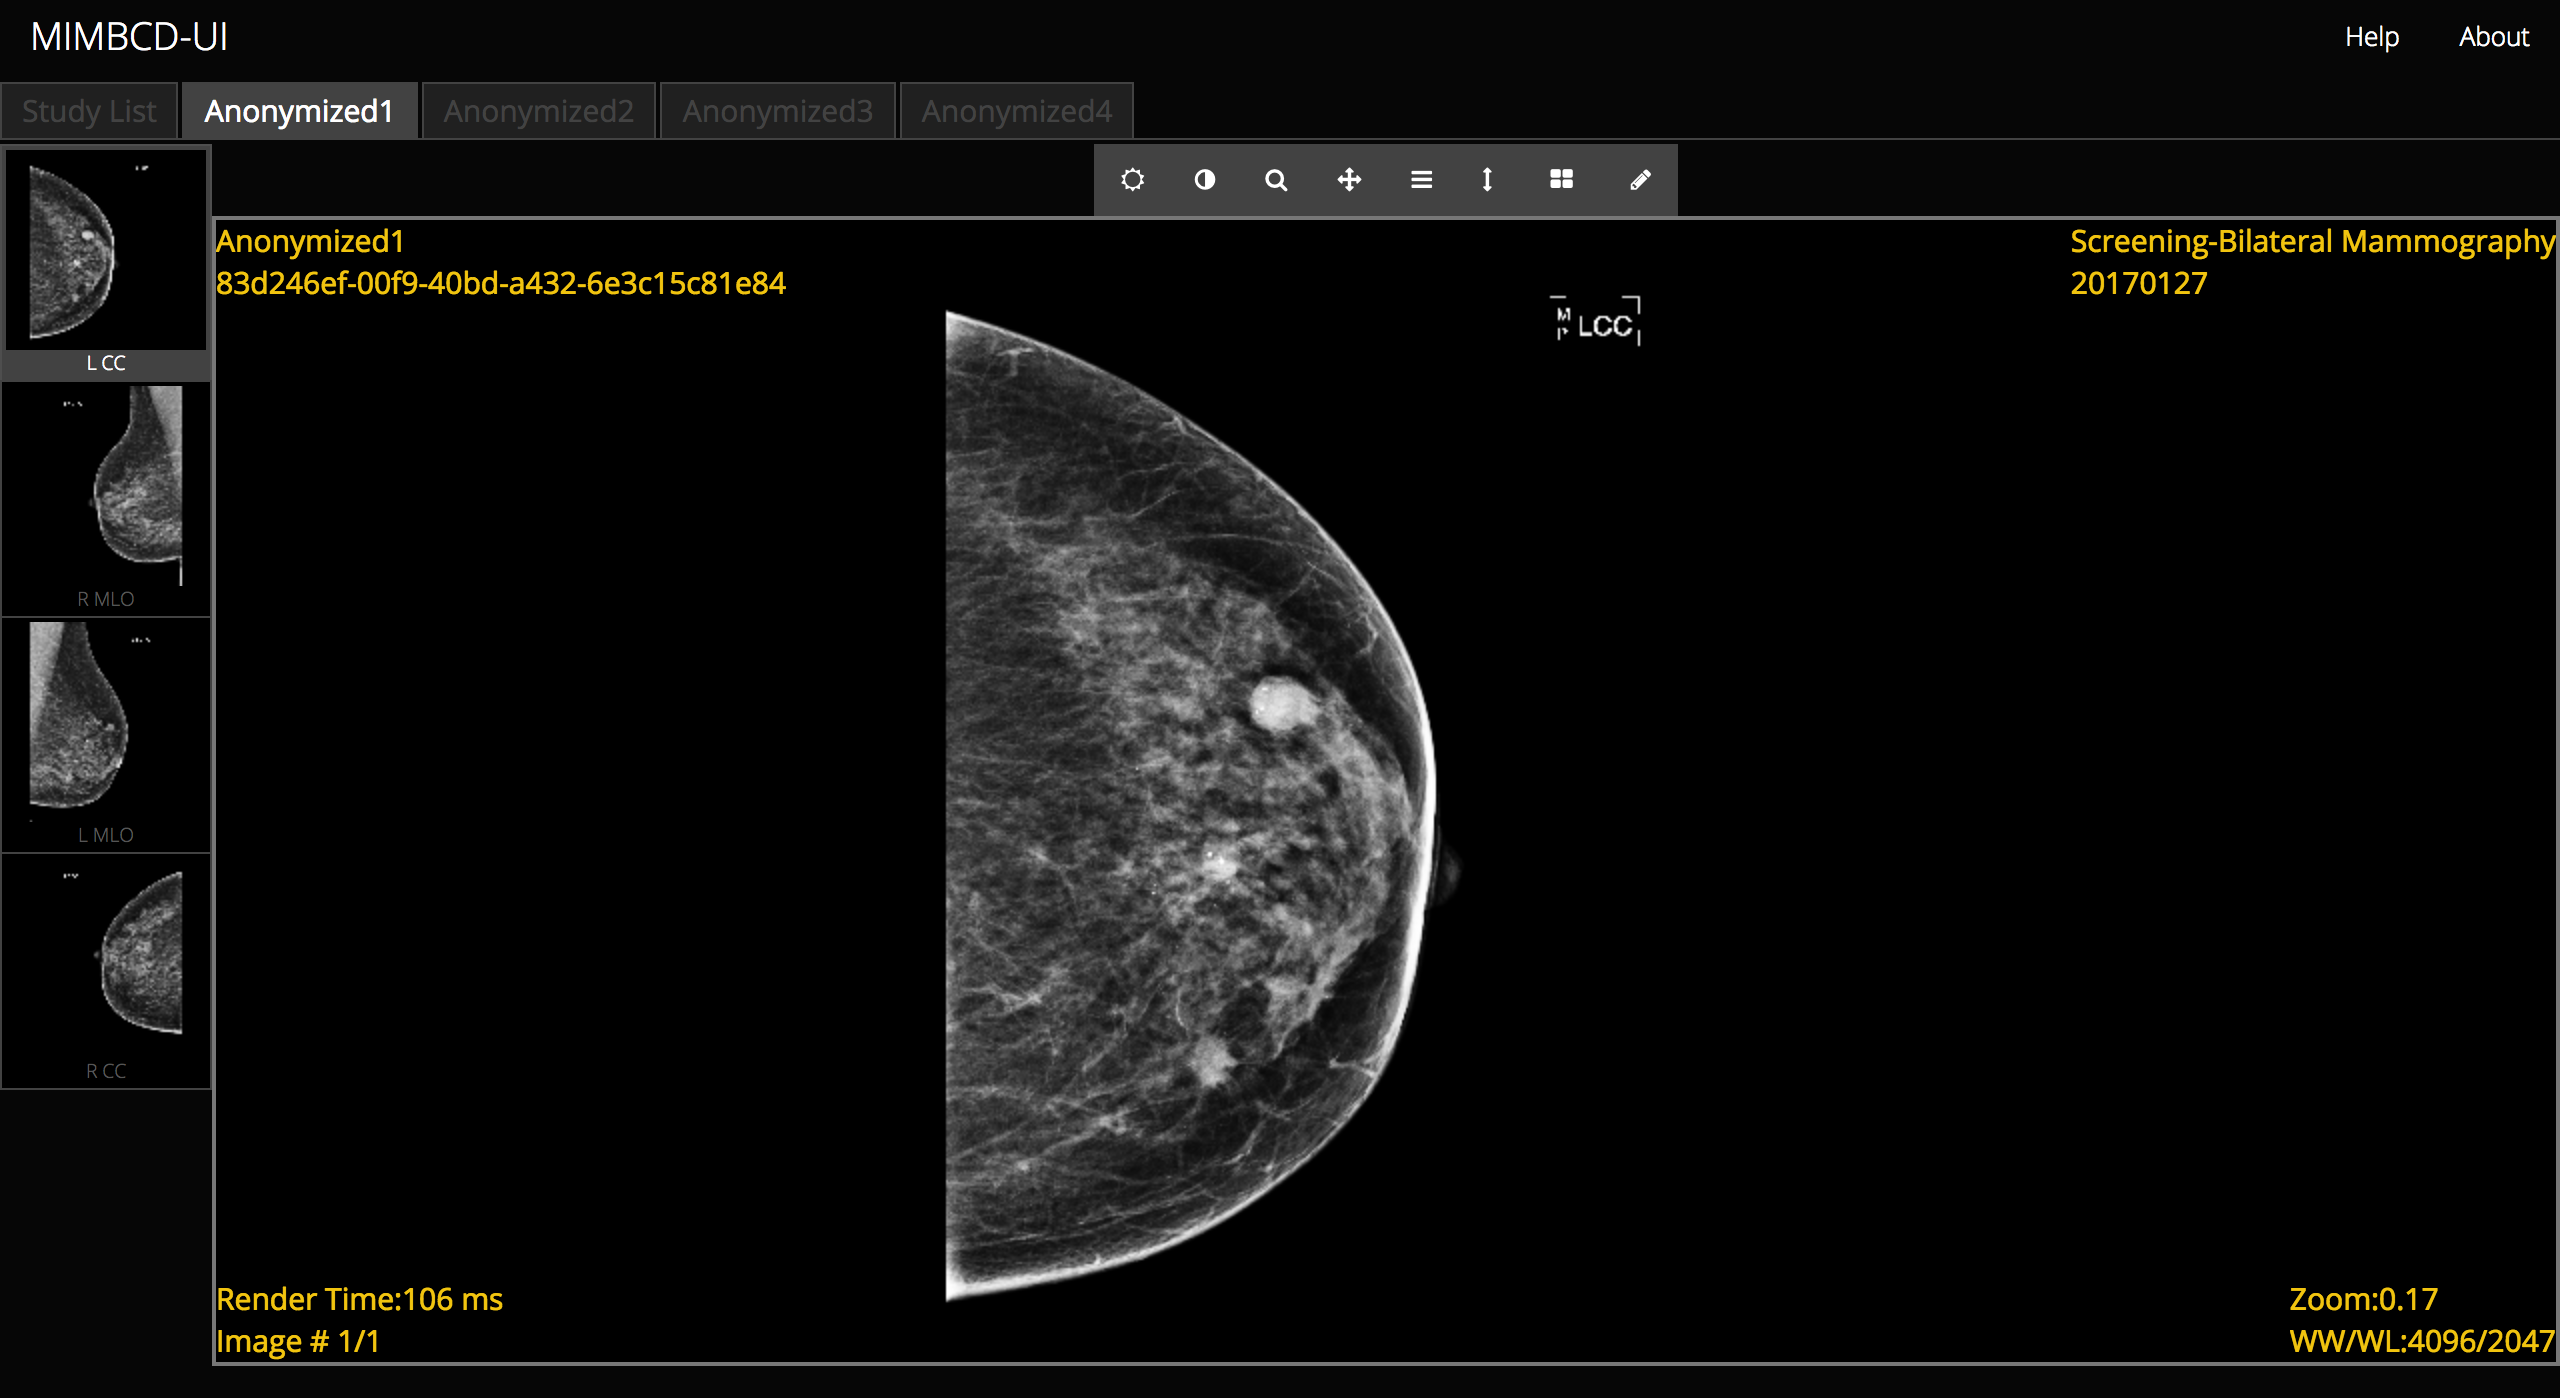
\includegraphics[width=\textwidth]{img1.png}
\end{figure}

As we can see on Figure 1, it describes our User Interface (UI), where the patient ("Anonymized1" for example) breast are on a small left column. The options are on a small row near of the viewport and are described bellow. We also have the tabs where the user can change the patient. The center viewport shows the DICOM Image and it can be configure to show a number up to four DICOM images. The viewport have some text information on it (yellow) with the details of the metadata.

Manual annotation is adopted by us thanks to the Cornerstone Freehand ROI Annotation feature. According to the Cornerstone Library, the user can create an annotation by setting up consecutive landmarks around a Region of Interest (ROI). The landmarks finish a lesion annotation when it interconnects othe landmark. Additional features available in our User Interface (UI) includes on-demand increment of the number of landmarks, and throw transformations of the shape of an annotation.

\clearpage

\section{Interactive Buttons}

\begin{figure}[h]
\caption{All interactive buttons.}
\centering

\includegraphics[width=\textwidth]{img4.png}
\end{figure}

The systems have several buttons (Figure 2) that allows the user to interact or access to a set of user interface features. The buttons are (from left to right):

\begin{itemize}
  \item WW/WC
  \item Invert
  \item Zoom
  \item Pan
  \item Stack Scroll
  \item Length Measurement
  \item Window Controller
  \item Freehand
\end{itemize}

The first feature, WW/WC button, will adjust the DICOM image luminosity, where this luminosity is controlled by activating the button and then by moving the mouse horizontally in north and south directions. The second feature, Invert button, will invert the pixels. The third feature is the Zoom, where the user can Zoom In and Zoom Out depending the direction of the mouse when the button is activated, also as WW/WC feature, the user can Zoom In by moving the mouse to south direction, and Zoom Out by moving the mouse to north direction. The fourth feature, Pan button, gives the user a free way to move the DICOM image inside the view, where the user just need to activate the feature and freely move the image. The fifth, Stack Scroll button, the gives the user the opportunity to change the frames, where the user just need to horizontally change the image by selecting the image and moving the mouse from north to south, and vice versa. The Length Measurement, is our sixth feature, where the user can measure inside the DICOM image. The seventh feature, Window Controller, gives the user the opportunity to select and manage many images to the viewport, is here where the user can configure the viewport with the 1x1, 2x1, 1x2 and 2x2 options. Last but not least, the eighth feature, Freehand, our most important, where the user can draw the annotation of the lesions.

\clearpage

\section{Procedures}

Each test will take place according to the following structure:

\subsection{Initial Questionnaire}

Prior to the start of the session, participants will be asked to complete a short questionnaire, with the aim of defining their user profile and experience with stereoscopic and other strives. The user will be asked to answer the following questions:

\begin{itemize}
  \item Sex, Age, Literacy.
  \item Experience with multi-touch devices (smartphones, tablets, etc).
  \item Experience with Picture Archiving and Communication System (PACS) and if so, which ones.
  \item Experience with Computer-aided Diagnosis (CAD) software and if so, which ones.
\end{itemize}

\subsection{Introduction}

A presentation of the systems and their use and capabilities will be made. They will be presented interactions and will be explained how to interact with the prototype, explaining the limitations.

\subsection{Training Session}

The user will be shown how to annotate and interact in all degrees of freedom. With the aim of enabling users to get their work done before the test tasks. This one training period will be less then 5 minutes.

\subsection{Execution of Tasks}

Throughout the test session, the user will perform freehand ROI annotation tasks in a traditional environment (mouse and keyboard). The session will thus be divided into two steps, during which the user will perform 4 tasks:

1) Access the prototype and observe the 4 tabs.

2) Go to "Anonymized1" patient, select the "L CC" image, and annotate the lesion.

3) Go to the patient "Anonymized2", select the first "MG" image and annotate the lesion.

4) Now go to the patient "Anonymized4", select the "US" image and annotate the lesion.

The task ends when the user understands that he/she has performed the proposed task, or when this is prolonged for a time beyond reasonable.

\subsection{Final Survey}

After completion of the tasks, users will be asked to complete a questionnaire to classify the prototype and technique according to various parameters such as ease of interaction, annotation, fun, etc.

\section{Tasks}

For the accomplishment of the tasks the objects visible in Figure 3 are used. These were chosen, so that there is only one possible way of being annotated, with only the white freehand draw annotation.

\begin{figure}[h]
\caption{User Interface Options}
\centering
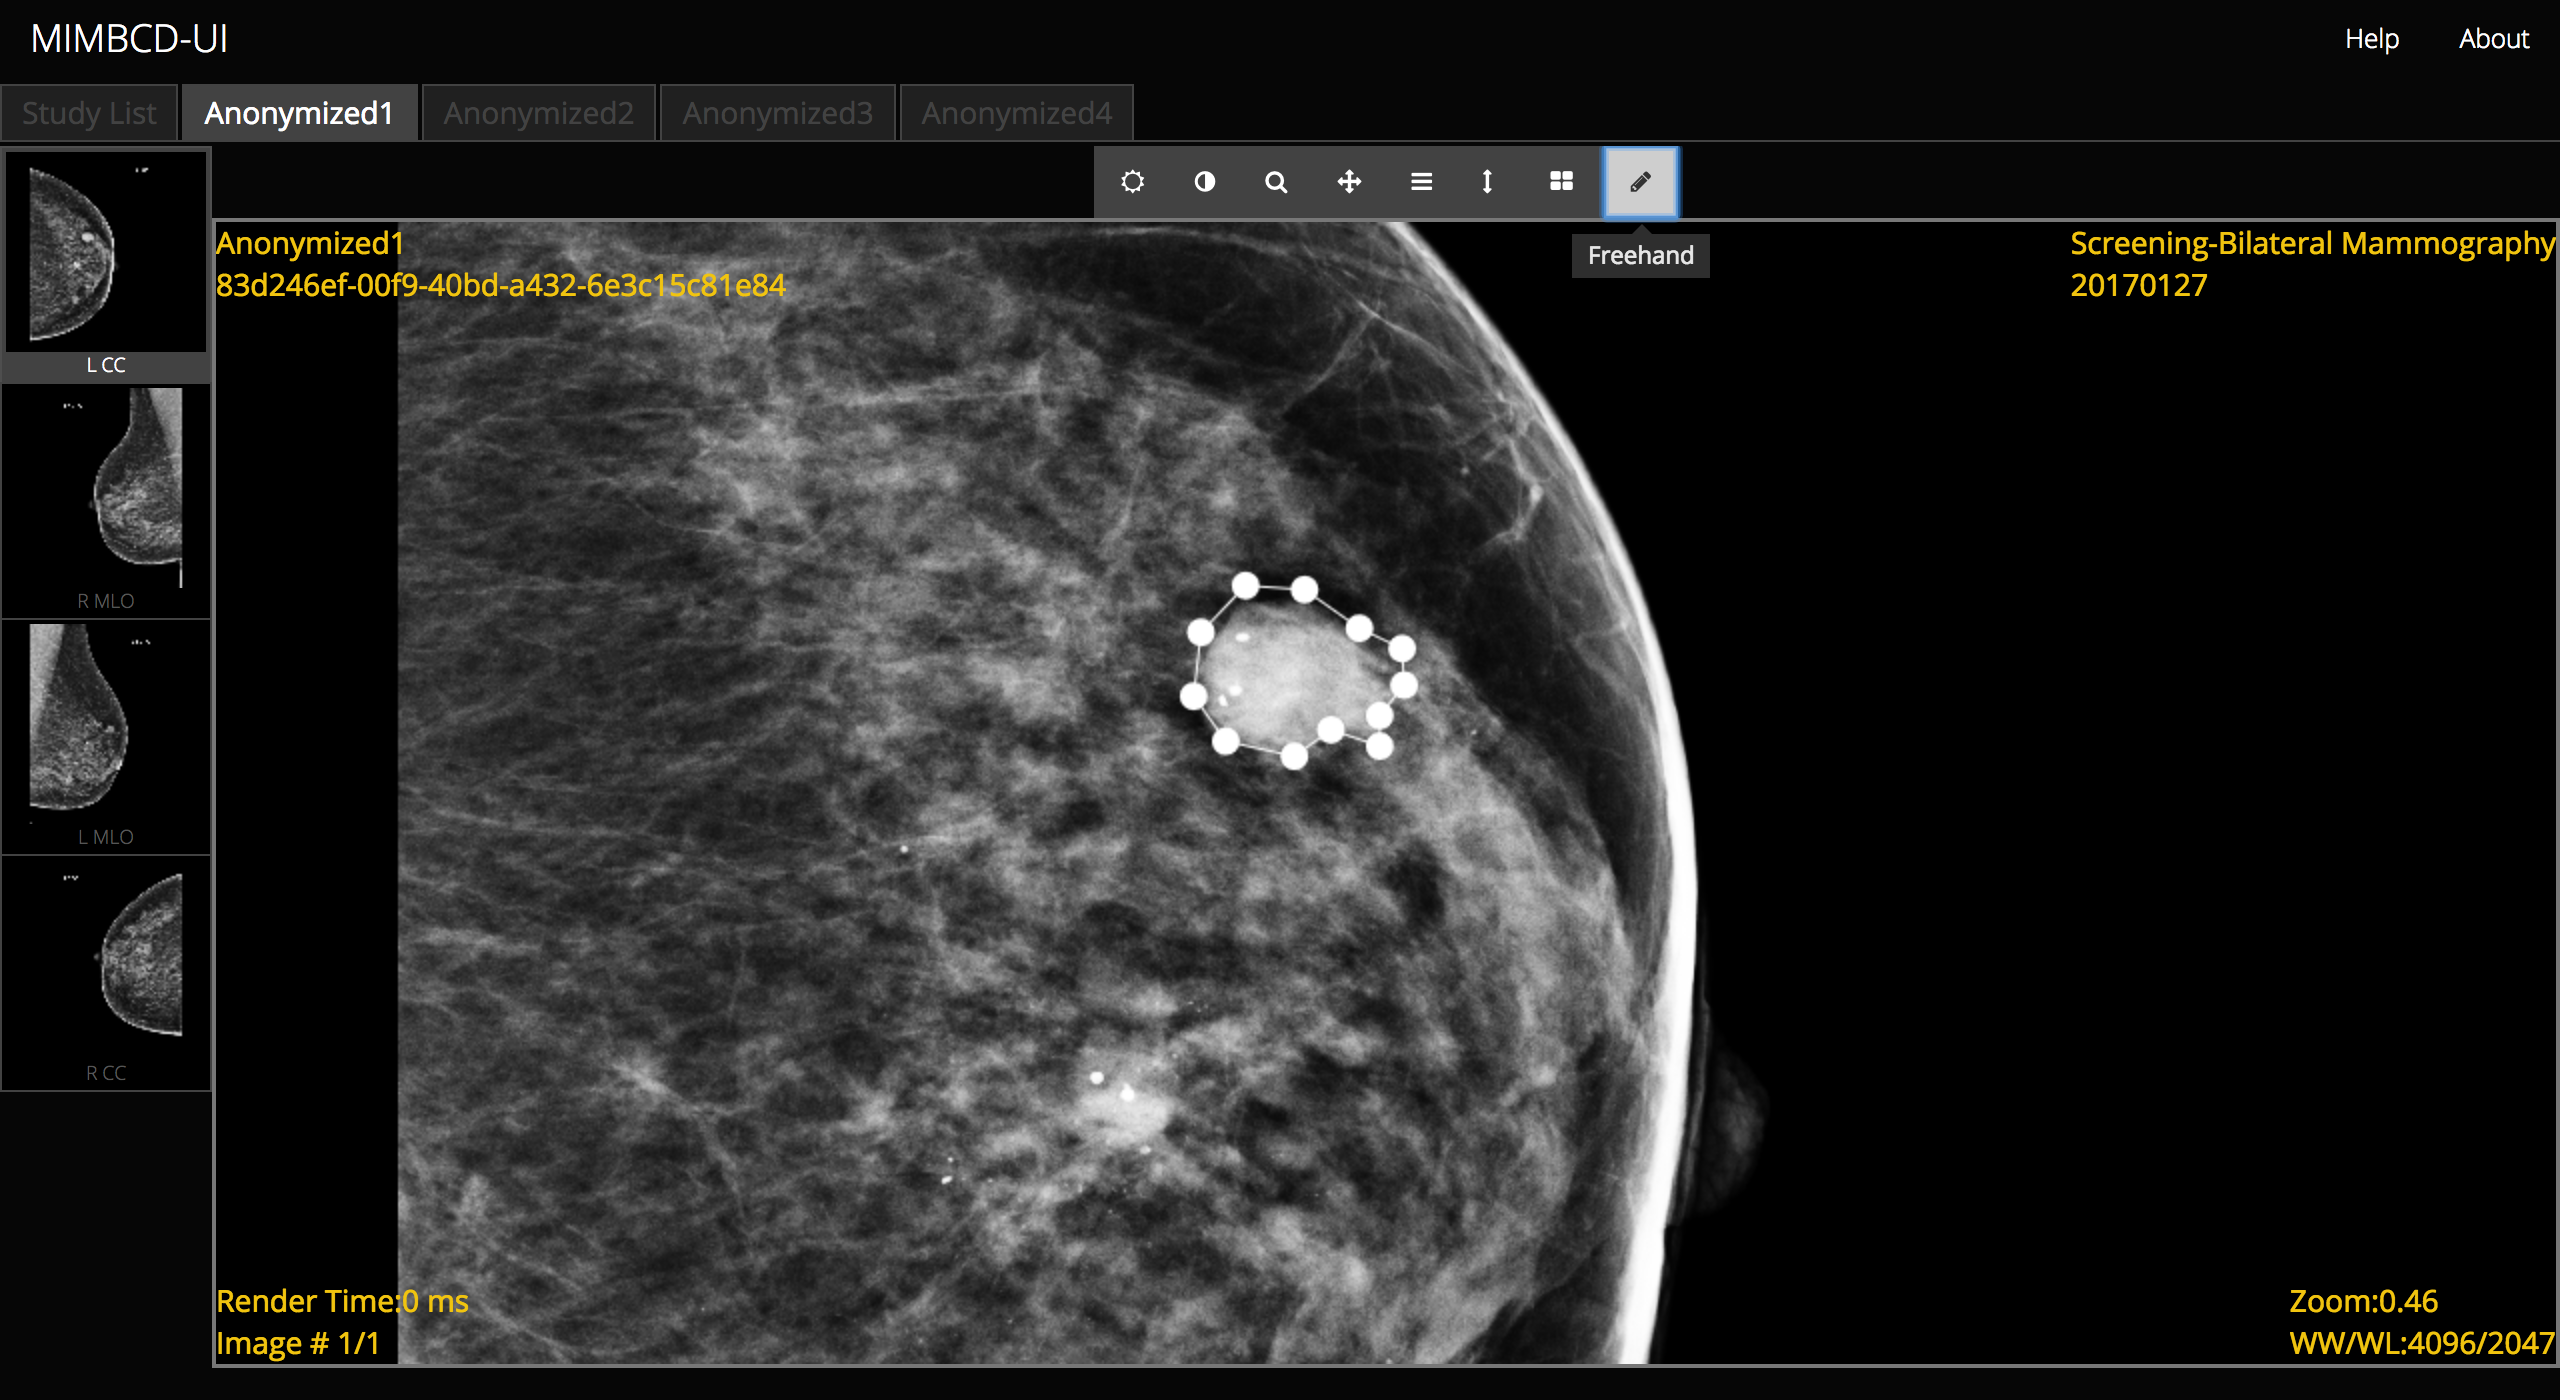
\includegraphics[width=\textwidth]{img2.png}
\end{figure}

The tasks in each environment will be executed in incremental difficulty order. In the first task the user only needs to observe and do some basic interaction throw a simple and small lesion, in the second task it is necessary to activate annotate a bigger lesion and harder one. Finally, on the third task to draw it on the hardest lesion we have. While in the last tasks we won't give the user information about how to do it, just say the patient and the image, while the lesion is also hard.

\clearpage

\section{Measurements}

The tests are intended to achieve the following measures:

\begin{itemize}
  \item Time measurement;
  \item Number of clicks;
  \item Number of errors;
  \item Efficiency;
  \item Difficulty;
  \item Experience;
\end{itemize}

Through the questionnaire after the test session, we intend to obtain the answers to the following questions for each environment (for each response a scale of 1 to 5 is given):

\begin{itemize}
  \item Difficulty of interaction.
  \item Difficulty translating.
  \item Difficulty performing a freehand ROI.
  \item Degree of interaction fun.
\end{itemize}

\end{document}